\documentclass[a4j]{jarticle}
\title{多体問題レポート3}
\author{35196004 天野智仁}
\usepackage{amsmath}	% required for `\align*' (yatex added)
\usepackage{listings}	% required for `\lstlisting' (yatex added)
\lstset{
  basicstyle={\ttfamily},
  identifierstyle={\small},
  commentstyle={\smallitshape},
  keywordstyle={\small\bfseries},
  ndkeywordstyle={\small},
  stringstyle={\small\ttfamily},
  frame={tb},
  breaklines=true,
  columns=[l]{fullflexible},
  numbers=left,
  xrightmargin=0zw,
  xleftmargin=3zw,
  numberstyle={\scriptsize},
  stepnumber=1,
  numbersep=1zw,
  lineskip=-0.5ex
}


\usepackage[dvipdfmx]{graphicx}	% required for `\includegraphics' (yatex added)
\begin{document}
\maketitle
\section{CG法の実装}
CG法の実装には,CG3法を用いた.コードは図に示した通りであり,はじめに行列$A$およびベクトル$b$を手入力した後,$A$が正値対称行列であることを確認した後,CG法を実行する流れになっている.

\begin{lstlisting}
 #CG Method

 #import
 import numpy as np

 #coefficient matrixA
 A=np.array([[10.5,1.5321,3.11111,-4.0546,-3.23],
           [1.5321,10,4,5,1],
           [3.11111,4,10,3,2],
           [-4.0546,5,3,10,4],
           [-3.23,1,2,4,10]])

 #coefficient matrixb
b=np.array([[2.3241],[3.4943],[4.5065],[5.6935],[6.2176]])

#order check of A
if A.shape[0]==A.shape[1]:
    print('the order of A is ',A.shape[0])
else:
    print('error::A is not a square matrix')
    exit(1)
    
    
#order check of B
if A.shape[0]==b.shape[0]:
    print(A.shape[0],'the order of B match with that of A ')
else
    print('error::'the order of B DOSE NOT match with that of A ')
    exit(1)


#order of A
size=A.shape[0]
num=size*size

#symmetry check of A
if np.sum(A.T==A)==num:
    print('A is symmetric')

#positive value check of A

D, O = np.linalg.eig( A )
print(D)
print(O)


testcounter=1

for i in range(size-1):
    if D[i] > 0:
        testcounter+=1

if testcounter==size:
    print('A is positive value matrix')
else:
    print('A is NOT  positive value matrix')
    exit(1)

#cg method initialize
x_0=np.array([[0],[0],[0],[0],[0]])
r_0=b-np.dot(A,x_0)
p_0=r_0

#convergence
delta=0.00001



#iteration num
count=0

#initialize
r=r_0
p=p_0
x=x_0

while np.linalg.norm(r, ord=2) > delta:
    y=np.dot(A,p)
    alpha=np.dot(r.T,r)/np.dot(p.T,y)
    xx=x+alpha*p
    rr=r-alpha*y
    beta=np.dot(rr.T,rr)/np.dot(r.T,r)
    pp=rr+beta*p
    
    x=xx
    r=rr
    p=pp
    count+=1
    if count%1==0:
        print(count)
        print(np.linalg.norm(r, ord=2))
 
#result
print(x)
print(count)
\end{lstlisting}


\section{CG法の実行}
実際に$5$次の正方行列$A$を選んで計算を実行した.選んだ行列$A$は
\begin{align*}
 A=\begin{pmatrix}\\
10.5&1.5321&3.11111&-4.0546&-3.23\\
           1.5321&10&4&5&1\\
           3.11111&4&10&3&2\\
           -4.0546&5&3&10&4\\
           -3.23&1&2&4&10
   \end{pmatrix}
\end{align*}
であり,ベクトル$b$は
\begin{align*}
 b=
\begin{pmatrix}
2.3241\\
3.4943\\
4.5065\\
5.6935\\
6.2176
\end{pmatrix}
\end{align*}
とした.この時行列$A$は正値対称であり,$b$は非ゼロ行列である.実装したプログラムによって得られた近似解は,収束判定$\delta=0.00001$において
\begin{align*}
x= 
\begin{pmatrix}
 0.71446122\\
 -0.16065586\\
 -0.04001816\\
  0.71515327\\
  0.59053888
 \end{pmatrix}
\end{align*}
であった.実際にこうして得られた$x$を用いて$Ax$を計算すると,ベクトル$b$に一致することが確認された.

次に,収束性について調べよう.CG法では原理的に(丸め誤差を無視すれば)係数行列のサイズ$N$以下の繰り返し回数で収束するはずである.実際,今回のケースでも繰り返し回数$5$回で収束しており,その収束の様子は図\ref{020034_28Jul19}に示すように,繰り返し$5$回目で激しく収束するような挙動を見せている.これは最後の繰り返しにおいて$5$個目の基底ベクトル$p_5$が得られたことによって解$x$を$5$つの基底ベクトルでよく表すことができるようになったためと解釈できる.
\begin{figure}[htb]
 \centering
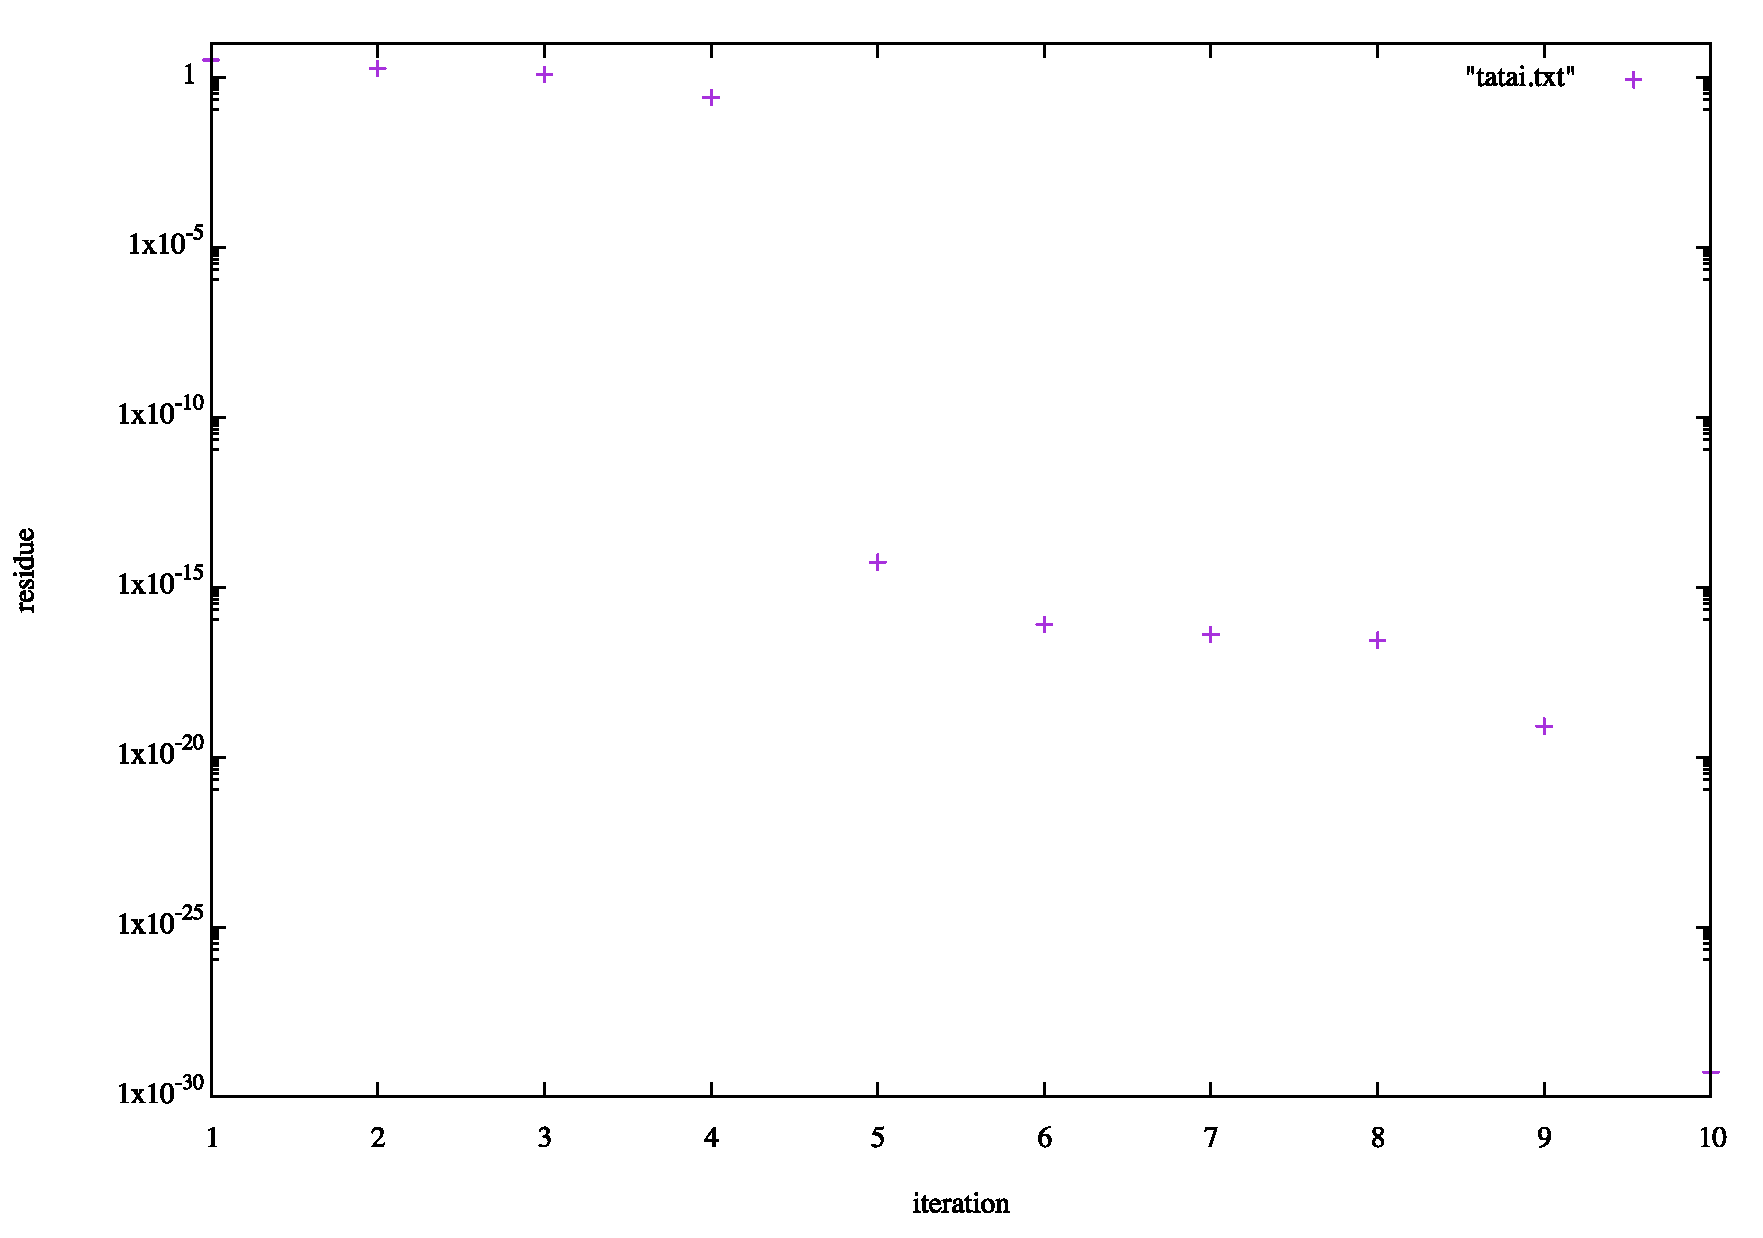
\includegraphics[bb=6 12 829 574,width=10cm]{tatai.pdf}
\caption{CG法の収束の様子}
\label{020034_28Jul19}
\end{figure}





\section{LAPACKとの比較}
最後に,LAPACKで用いられている方法との比較を行う.LAPACKには連立方程式を解くための多数の方法が実装されているが,その中でもDPOSVという,実正値対称行列$A$および行列$B$に対して用いることができるアルゴリズムを利用した.このアルゴリズムでは,行列$A$のコレスキー分解
\begin{align*}
 A=LL^{\mathrm{T}}
\end{align*}
ただし$L$は下三角行列,に分解することで,方程式$Ax=B$の解を
\begin{align*}
 y&=L^{\mathrm{T}}x \\
 b&=Ly
\end{align*}
と分解して解く,と言うことをしている.

このアルゴリズムを動かすためのコードを図に示した.
\begin{lstlisting}
 include<math.h>
#include<stdio.h>
#define SIZE 5 

int main(void){

  int i,j;
  /* A */
  double A[SIZE][SIZE];
  A[0][0]=10.5;
  A[0][1]=1.5321;
  A[0][2]=3.11111;
  A[0][3]=-4.0546;
  A[0][4]=-3.23;
  A[1][1]=10.0;
  A[1][2]=4.0;
  A[1][3]=5.0;
  A[1][4]=1.0;
 A[2][2]=10.0;
  A[2][3]=3.0;
  A[2][4]=2.0;
  A[3][3]=10.0;
  A[3][4]=4.0;
  A[4][4]=10.0;

  for(i=0;i<SIZE;i++){
    for(j=i;j<SIZE;j++){
      A[j][i]=A[i][j];
    }
  }

  /* b */
  double b[SIZE];
  b[0]=2.3241;
  b[1]=3.4943;
  b[2]=4.5065;
  b[3]=5.6935;
  b[4]=6.2176;

  /* dposv */
  char UPLO='U';
  int  N=SIZE; 
  int NRHS=1; 
  int LDA=SIZE; 
  int LDB=SIZE; 
  int info;
  dposv(&UPLO,&N,&NRHS,&A,&LDA,&b,&LDB,&info);

  return 0;
}



\end{lstlisting}



全く同じ$A$および$b$に対してこのコードを実行した結果は
\begin{align*}
 x=
\begin{pmatrix}
    0.7144612167 \\
    -0.1606558645\\
    -0.0400181555\\
     0.7151532710\\
     0.5905388822
\end{pmatrix}
\end{align*}
となり,CG法によるものと得られている桁において一致している.こうして異なるアルゴリズムでも同じ結果が得られていることが確認できた.

\end{document}